% Fig 1A: the WNT--RA--HOX network, one edge per term of Eqs (1)-(7).
% Activation = blue arrow, repression = red bar (paper palette). Compile:
%   pdflatex fig01a_network.tex
\documentclass[border=2pt]{standalone}
\usepackage{tgheros}
\renewcommand{\familydefault}{\sfdefault}
\usepackage[T1]{fontenc}
\usepackage{sansmath}
\usepackage{tikz}
\usetikzlibrary{arrows.meta,positioning,calc,shapes.geometric}
\definecolor{act}{HTML}{1F77B4}
\definecolor{rep}{HTML}{CC3333}
\definecolor{ink}{HTML}{1A1A1A}
\definecolor{inp}{HTML}{EDEDED}
\definecolor{dis}{HTML}{FF7F0E}
\begin{document}
\sansmath
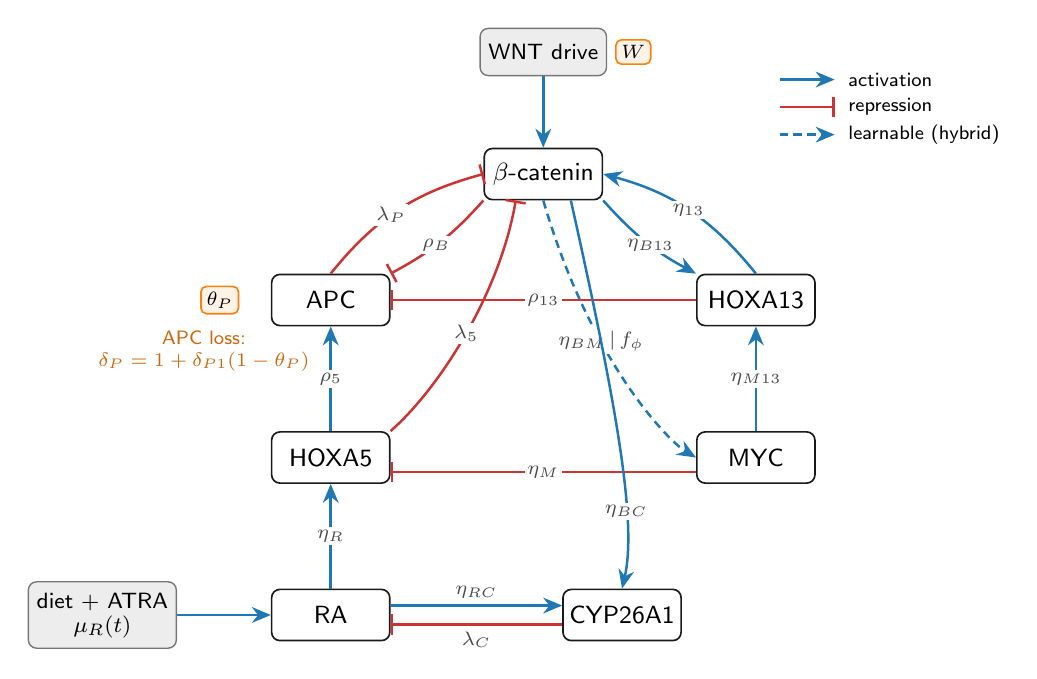
\begin{tikzpicture}[font=\sffamily\small,
  st/.style={draw=ink, line width=0.6pt, rounded corners=3pt, fill=white,
             minimum width=15mm, minimum height=6.5mm, inner sep=2pt},
  inp/.style={draw=ink!60, line width=0.5pt, rounded corners=3pt, fill=inp,
             minimum height=6mm, inner sep=3pt, font=\sffamily\footnotesize},
  a/.style={-{Stealth[length=2.4mm,width=2mm]}, line width=0.9pt, color=act},
  r/.style={-{Bar[width=2.6mm]}, line width=0.9pt, color=rep},
  lab/.style={font=\sffamily\scriptsize, inner sep=1pt, fill=white, text=ink!80},
  par/.style={draw=dis, line width=0.6pt, rounded corners=2pt, fill=dis!10,
              font=\sffamily\scriptsize, inner sep=2pt}]
% nodes
\node[inp]  (W)   at (0,  1.55) {WNT drive};
\node[st]  (b)   at (0,  0)    {$\beta$-catenin};
\node[st]  (p)   at (-2.7,-1.6){APC};
\node[st]  (h13) at (2.7, -1.6){HOXA13};
\node[st]  (h5)  at (-2.7,-3.6){HOXA5};
\node[st]  (m)   at (2.7, -3.6){MYC};
\node[st]  (r)   at (-2.7,-5.6){RA};
\node[st]  (c)   at (1.0, -5.6){CYP26A1};
\node[inp]  (mu)  at (-5.6,-5.6){\begin{tabular}{@{}c@{}}diet + ATRA\\[-1pt]$\mu_R(t)$\end{tabular}};
% disease parameters
\node[par, right=1mm of W] {$W$};
\node[par, left=4mm of p] (thp) {$\theta_P$};
% edges: beta-catenin equation
\draw[a] (W) -- (b);
\draw[a] (h13.north) to[bend right=18] node[lab, pos=0.5]{$\eta_{13}$} (b.east);
\draw[r] (p.north) to[bend left=18] node[lab, pos=0.45]{$\lambda_P$} (b.west);
\draw[r] (h5.north east) .. controls (-1.3,-2.7) and (-0.55,-1.5) .. node[lab, pos=0.5]{$\lambda_5$} ([xshift=-3.5mm]b.south);
% APC equation
\draw[r] (b.south west) to[bend left=10] node[lab, pos=0.55]{$\rho_B$} (p.north east);
\draw[a] (h5) -- node[lab]{$\rho_5$} (p);
\draw[r] (h13.west) -- node[lab, pos=0.5]{$\rho_{13}$} (p.east);
% HOXA13
\draw[a] (b.south east) to[bend right=10] node[lab, pos=0.55]{$\eta_{B13}$} (h13.north west);
\draw[a] (m) -- node[lab]{$\eta_{M13}$} (h13);
% MYC (the main learned edge)
\draw[a, densely dashed] (b.south) .. controls (0.6,-2.4) and (1.6,-3.4) .. node[lab, pos=0.35]{$\eta_{BM}\,|\,f_\phi$} (m.west);
% HOXA5
\draw[r] (m.west|-m.south west) ++(0,0.15) -- node[lab, pos=0.5]{$\eta_M$} ([yshift=0.15cm]h5.south east);
\draw[a] (r) -- node[lab]{$\eta_R$} (h5);
% RA / CYP26A1
\draw[a] (mu) -- (r);
\draw[a] ([yshift=1.2mm]r.east) -- node[lab, above=0.4mm]{$\eta_{RC}$} ([yshift=1.2mm]c.west);
\draw[r] ([yshift=-1.2mm]c.west) -- node[lab, below=0.4mm]{$\lambda_C$} ([yshift=-1.2mm]r.east);
\draw[a] ([xshift=3.5mm]b.south) .. controls (0.9,-2.8) and (1.2,-4.4) .. node[lab, pos=0.7]{$\eta_{BC}$} (c.north);
% APC-loss annotation
\node[font=\sffamily\scriptsize, text=dis!80!black, align=center, below=0.8mm of thp, xshift=-2mm]
  {APC loss:\\ $\delta_P = 1+\delta_{P1}(1-\theta_P)$};
% legend
\begin{scope}[shift={(3.0,0.9)}]
\draw[a] (0,0.3) -- (0.7,0.3); \node[anchor=west, font=\sffamily\scriptsize] at (0.75,0.3) {activation};
\draw[r] (0,-0.05) -- (0.7,-0.05); \node[anchor=west, font=\sffamily\scriptsize] at (0.75,-0.05) {repression};
\draw[a, densely dashed] (0,-0.4) -- (0.7,-0.4); \node[anchor=west, font=\sffamily\scriptsize] at (0.75,-0.4) {learnable (hybrid)};
\end{scope}
\end{tikzpicture}
\end{document}
